% Source: Code/xband-radar-sim/docs/radar_simulation_technical.tex
% Description: Atmospheric attenuation vs range at X-band. At 50 km, two-way loss is about 1 dB.

\documentclass[border=4pt]{standalone}
\usepackage{algpseudocode}
\usepackage{amsmath,amssymb,amsfonts}
\usepackage[T1]{fontenc}
\usepackage{graphicx}
\usepackage{pgfplots}
\usepackage{tikz}
\usepackage{xcolor}
\pgfplotsset{compat=1.18}
\usetikzlibrary{arrows.meta,positioning,shapes.geometric,calc,patterns,decorations.pathmorphing,3d,angles,quotes}

\definecolor{radargreen}{RGB}{0,255,0}
\definecolor{raycolor}{RGB}{255,165,0}
\definecolor{targetcolor}{RGB}{255,0,0}
\definecolor{groundcolor}{RGB}{139,90,43}
\definecolor{skycolor}{RGB}{135,206,235}
\definecolor{beamcolor}{RGB}{255,255,0}


\begin{document}
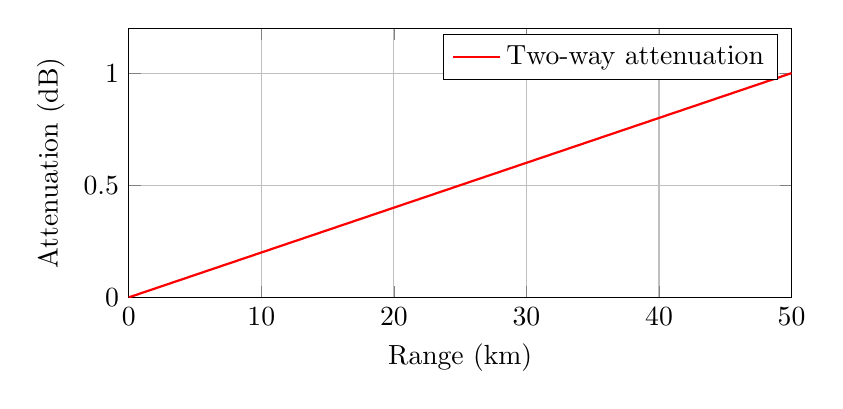
\begin{tikzpicture}
\begin{axis}[
    width=10cm, height=5cm,
    xlabel={Range (km)},
    ylabel={Attenuation (dB)},
    xmin=0, xmax=50,
    ymin=0, ymax=1.2,
    grid=both,
]
    \addplot[thick, red, domain=0:50] {0.01 * 2 * x};
    \addlegendentry{Two-way attenuation}
\end{axis}
\end{tikzpicture}
\end{document}
